\section{Webes keretrendszerek}
A keretrendszerek \cite{frameworks} napjainkban felkapott rendszerek lettek a felhasználók között. Ezek a rendszerek sokoldalúak, robusztusak és hatékonyak. A különböző alkalmazások fejlesztéséhez az ilyen jellegű rendszerek segítségével csak a magasabb szintű funkcionalitások elvégzésére kell koncentrálni. Erre az a magyarázat, hogy a keretrendszer gondoskodik az alacsonyabb funkcionalitásokról, amelyek már rengeteg tesztelt kódot tartalmaznak, így mi ezeket a funkcionalitásokat nem kell külön megírjuk és leteszteljük, hogy helyes-e a megírt kód. Számos előnyt lehet felsorolni, hogy miért jó ha használjuk ezeket a rendszereket.
\begin{itemize}
	\item Elősegíti a tervezési minták megfelelő kialakítását.
	\item Biztonságosabb kódolás.
	\item A redundáns kód elkerülése.
	\item Következetes kódfejlesztés kevesebb hibával.
	\item Megkönnyíti a kód tesztelését és a hibakeresést is.
	\item Az alkalmazás fejlesztéséhez szükséges idő lecsökken.
\end{itemize}

Az \ref{fig:fornt_frameworks} ábrán látható egy rangsorolás a Github és Stack Overflow által készített pontozások alapján a Front-end-et megvalósító keretrendszereknek. Látható hogy az első helyen a React van összesített 98 ponttal. A második helyen áll az ASP.NET MVC 95 ponttal viszont itt észlelhető az is, hogy a Githubról nem jött pontozás erről a keretrendszerről. Az ábrán látható további keretrendszerek úgyan annyi összpontozást kaptak. Az ábra alapján a legjobb döntés egy webes keretrendszer választásra a React lenne visszont a többi keretrendszer sincs sokkal lemaradva az első helyezettől.
\begin{figure}[H]
	\centering
	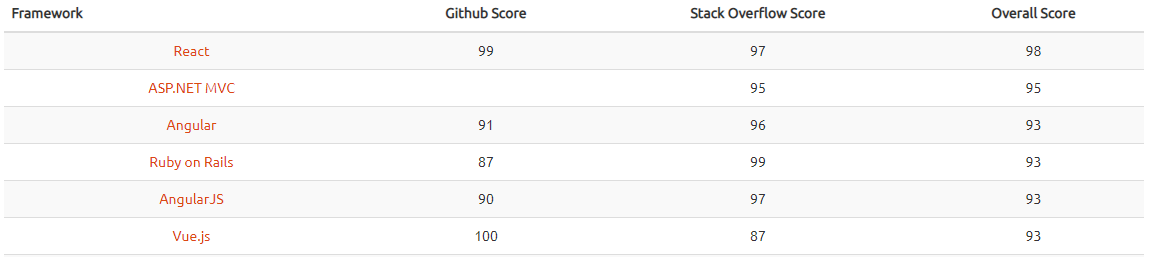
\includegraphics[width=1\linewidth]{figures/images/vueang.png}
	\caption[Webes keretrendszerek Github és Stack Overflow pontozások alapján]{\textit{Webes keretrendszerek Github és Stack Overflow pontozások alapján}\footnotemark}
	\label{fig:fornt_frameworks}
\end{figure}
\footnotetext{http://hotframeworks.com/}

2021-ben a 10 leghasználatosabb Back-end keretrendszer a Spring - Spring Boot, NodeJS, Laravel, Django, Flask, Ruby, Play, Asp.Net, CakePHP és Symphony.\cite{backendframework1}\cite{backendframework2} 

A keretrendszerek világa igen nagy így a következőkben olvashatunk részletesebben néhány keretrendszerről mint például: az Angular, Vue.js, Spring Boot és a NodeJs.

\subsection{Angular}
A Google munkatársai 2008-ban fejlesztettek a JavaScript alapú Angular keretrendszert \cite{wohlgethan2018supportingweb}.Abban az időben a webhelyek zöme többoldalas alkalmazás megközelítésén alapult. A több oldalas alkalmazások lassúnak bízonyultak így bevezették az egy oldalas alkalmazásokat. Az egy oldalas alkalmazások abban jobbak a több oldalas alkalmazásoknál, hogy weboldal betöltése folyamán nem kell mindig mindent újra betölteni, hanem csak azok a részek töltődnek be ahol változások fognak megjelenni. Az Angular volt az egy oldalas alkalmazások első kerete. Az egyik fő előnye, hogy a felhasználók egyszerű struktúrával kell dolgozzanak. Megtanulják az Angular sajátos felépítését ezáltal gyorsan és optimálisabban tudnak benne fejleszteni. Az sem elhanyagolható, hogy a fejlesztők egy részletes és egyértelmű dokumentációval szolgáltak a felhasználóknak.

\subsection{Vue.js}
A Vue.js (röviden: Vue) \cite{wohlgethan2018supportingweb} tekinthető az egyik legújabb keretrendszernek. Hasonlít az Angularhoz. Mindkéttő TypeScript típusú. Használható kisebb, egyszerűbb projekteknél. Mindig egy oldalas alkalmazásokat lehet benne elkészíteni ami a felhasználói élmányt segíti elő. Fő érdeme a skálázhatóság. Különlegessége, hogy egy nyílt forráskódú közösség fejlesztette ki, nem pedig egy nagyobb vállalat. Komponens alapú keretrendszer amely azt jelenti, hogy komponenseket különböztetünk és jelenítünk meg. Egy komponensen belül tudunk írni HTML, CSS és Script elemeket is. A megjelenítés egy oldalon történik ezért szükséges használni a útválasztást (rout).
	
\subsection{Angular vs Vue.js}
Mindkét keretrendszernek megvannak az előnyei \ref{tab:table1} táblázat és a hátrányai is \ref{tab:table2} táblázat. 
\begin{table}[H]
	\begin{footnotesize}
		\begin{center}
			\caption[Előnyök Angular és Vue.js között]{\textit{Előnyök Angular és Vue.js között \cite{vuevsang}}}
			\label{tab:table1}
			\begin{tabular}{p{0.5cm}|p{6cm}|p{6cm}}
				\textbf & \textbf{Angular} & \textbf{Vue.js}\\
				\hline
				1 & TypeScript használata & TypeScript használata, részletes dokumentáció\\
				\hline
				2 & Részletes dokumentációval rendelkezik & Egy oldalas alkalmazások készítése \\
				\hline
				3 & Gyorsítja a fejlesztést & Könnyű integráció a meglévő struktúrákba \\
				\hline
				4 & & Kihasználja virtuális DOM előnyeit \\
				\hline
				5 & & Sebessége és rugalmassága optimális \\
			\end{tabular}
		\end{center}
	\end{footnotesize}
\end{table}
\begin{table}[H]
	\begin{footnotesize}
		\begin{center}
			\caption[Hátrányok Angular és Vue.js között]{\textit{Hátrányok Angular és Vue.js között \cite{vuevsang}}}
			\label{tab:table2}
			\begin{tabular}{p{0.5cm}|p{6cm}|p{6cm}} 
				\textbf & \textbf{Angular} & \textbf{Vue.js}\\
				\hline
				1 & Számos különféle struktúrát kínál, nehezíti a tanulást & Kevesebb erőforrást kínál\\
				\hline
				2 & Lassabb teljesítmény mert működik a reális DOM &  \\
			\end{tabular}
		\end{center}
	\end{footnotesize}
\end{table}

\subsection{NodeJs}
A NodeJs \cite{js2016node} egy olyan szoftver platform, amely a Chrome V8 JavaScript futási idején épül fel. Fontos tulajdonsága, hogy skálázható ezért is sokan használják. Eseményvezérelt, nem blokkoló I/O modellt használ, amely könnyűvé és hatékonnyá teszi a valós idejű alkalmazások megvalósítását, amelyek elosztott rendszeren futnak át. Tulajdonképpen közvetlenül a natív gépi kódra fordítja le a JavaScript-et, amelyenek hatására az adatformátum egy lépése megszűnik, ezzel növelve az alkalmazás sebességét. Legtöbb esetben a NodeJs használatakor adatbázisnak NoSQL adatbázisokat választanak.

NodeJs a következő különlegességeket tartalmazza \cite{nodejsspring}:
\begin{itemize}
	\item A NodeJS alkalmazások fejlesztésének elindítása könnyű.
	\item Az agilis fejlesztési módszertant követi, amely alkalmas a nagyon skálázható alkalmazásfejlesztési szolgáltatásokra.
	\item Nagy projekteknél gyorsabban működik mint a Java.
	\item Hatalmas erőforrás-készlet könyvtárakkal rendelkezik
\end{itemize}
	
\subsection{Spring Boot}
A Spring Boot \cite{jovanovic2017java} célja a Spring alkalmazás fejlesztés egyszerűsítése. Megtalálhatóak benne a következő tulajdonságok:
\begin{itemize}
	\item Automatikus konfigurációk - Az alkalmazások Springként való működése érdekében.
	\item Indítófüggőségek - Biztosítja a felhasználóknak a szükséges függőségek(dependency) beimportálását. Ilyen lehet a Maven, Hibernate validátor, adatbázis eléréseket stb.
	\item Parancssori tolmács.
	\item Működtetés - A console-ba megjelennek az alkalmazás működésével kapcsolatos információk. Ilyen információ lehet a hiba, az elvégzett művelet stb.
\end{itemize}
	
Radikálisan gyorsabb és széles körben hozzáférhető, érthető Spring fejlesztést nyújt. Számos funkciót kínál: beágyazott szervereket, metrikákat, ellenőrzéseket, külső konfigurációkat. Saját struktúrával rendelkezik és nem tesz különbséget az adatbázisok között. A JAVA nyelvet használja.

Spring Boot a következő különlegességeket tartalmazza \cite{nodejsspring}:
\begin{itemize}
	\item Egyszerű, minden eszköz és operációs rendszer támogatja.
	\item Beépített nyelvbiztonsági funkciókkal rendelkezik, amelyeket a Java Compiler beágyaz.
	\item Robusztus kódot alkalmaz.
	\item Integrációs képesség jó.
	\item Beágyazott HTTP-kiszolgálókat, például Jetty, Tomcat használ és egyszerűen teszteli a webes alkalmazásokkal.
\end{itemize}

\subsection{Spring Boot vs NodeJs}

A Spring Boot és a NodeJs közötti néhány előnyt \cite{nodespringcomp} az \ref{tab:tableSpringNodeJsPros} táblázatban tudjuk megtekinteni.
\begin{table}[H]
	\begin{footnotesize}
		\begin{center}
			\caption[Előnyök Spring Boot és NodeJS között]{\textit{Előnyök Spring Boot és NodeJS között}}
			\label{tab:tableSpringNodeJsPros}
			\begin{tabular}{p{0.5cm}|p{6cm}|p{6cm}}
				\textbf & \textbf{Spring Boot} & \textbf{NodeJs}\\
				\hline
				1 & Java nyelv már nagyon ismeretes így ha elakadás van könnyű segítséget kérni/keresni& A JavaScript futásidejének köszönhetően gyors az adatfeldolgozásban\\
				\hline
				2 & Többszálú programozás & Memória takarékos\\
				\hline
				3 & Nagyszámú erőforrás áll rendelkezésre (például: az autentikáció már előre megvan írva) & NPM (Node Package Manager) -nek köszönhetően egyre több szolgáltatás érhető el. \\
			\end{tabular}
		\end{center}
	\end{footnotesize}
\end{table}

Minden keretrendszer között találhatunk előnyöket is meg hátrányokat is. A Spring Boot és a NodeJs között előnyöket az \ref{tab:tableSpringNodeJsPros} táblázatban már tárgyaltuk. A következőkbe néhány hátrányról \cite{nodespringcomp} lesz szó: 
\begin{itemize}
	\item A NodeJS nem tud hatékonyan teljesíteni nagy számítások esetén.
	\item A NodeJS mivel még új technika ezért még nincs teljesen kifelesztve, tesztelve így sok olyan hibába ütközhetünk amire nincs ideális megoldás.
	\item A Spring Boot legnagyobb hátránya, hogy a memóriaigénye nagyon nagy.
	\item A Spring Boot egy másik hátránya, hogy a hiba keresés meglehetősen nehéz mivel sok beépített kód található benne.
\end{itemize}

Összefoglalva mindkét technológia a maga módján megfelelő különböző alkalmazások tervezésénél. Ha az alkalmazás sok bemeneti/kimeneti feladatot (például: sok regisztráció) tartalmaz akkor mindenképp a NodeJs-t érdemes választani. Viszont ha biztonságos és önálló alkalmazást tervezünk amely intenzív CPU használatot igényel akkor a Spring Boottal érdemes foglalkozni.